\section{Design and Implementation} \label{sec:4}

We begin by providing an overview of page fault handling in CheriBSD~\cite{cheribsd} to illustrate how CHERI-picking fits into the existing code. Traditional prefetchers rely on memory access history, which is accessible at page fault time, whereas CHERI-picking relies on the \emph{contents} of memory pages, which is available only after a page has been swapped in. This algorithmic difference produces a rather different implementation described in ~\autoref{sec:DI_CP_Policy}.

\subsection{CheriBSD swap workflow}
\label{sec:DI_swap}

\begin{figure}[]
\centering
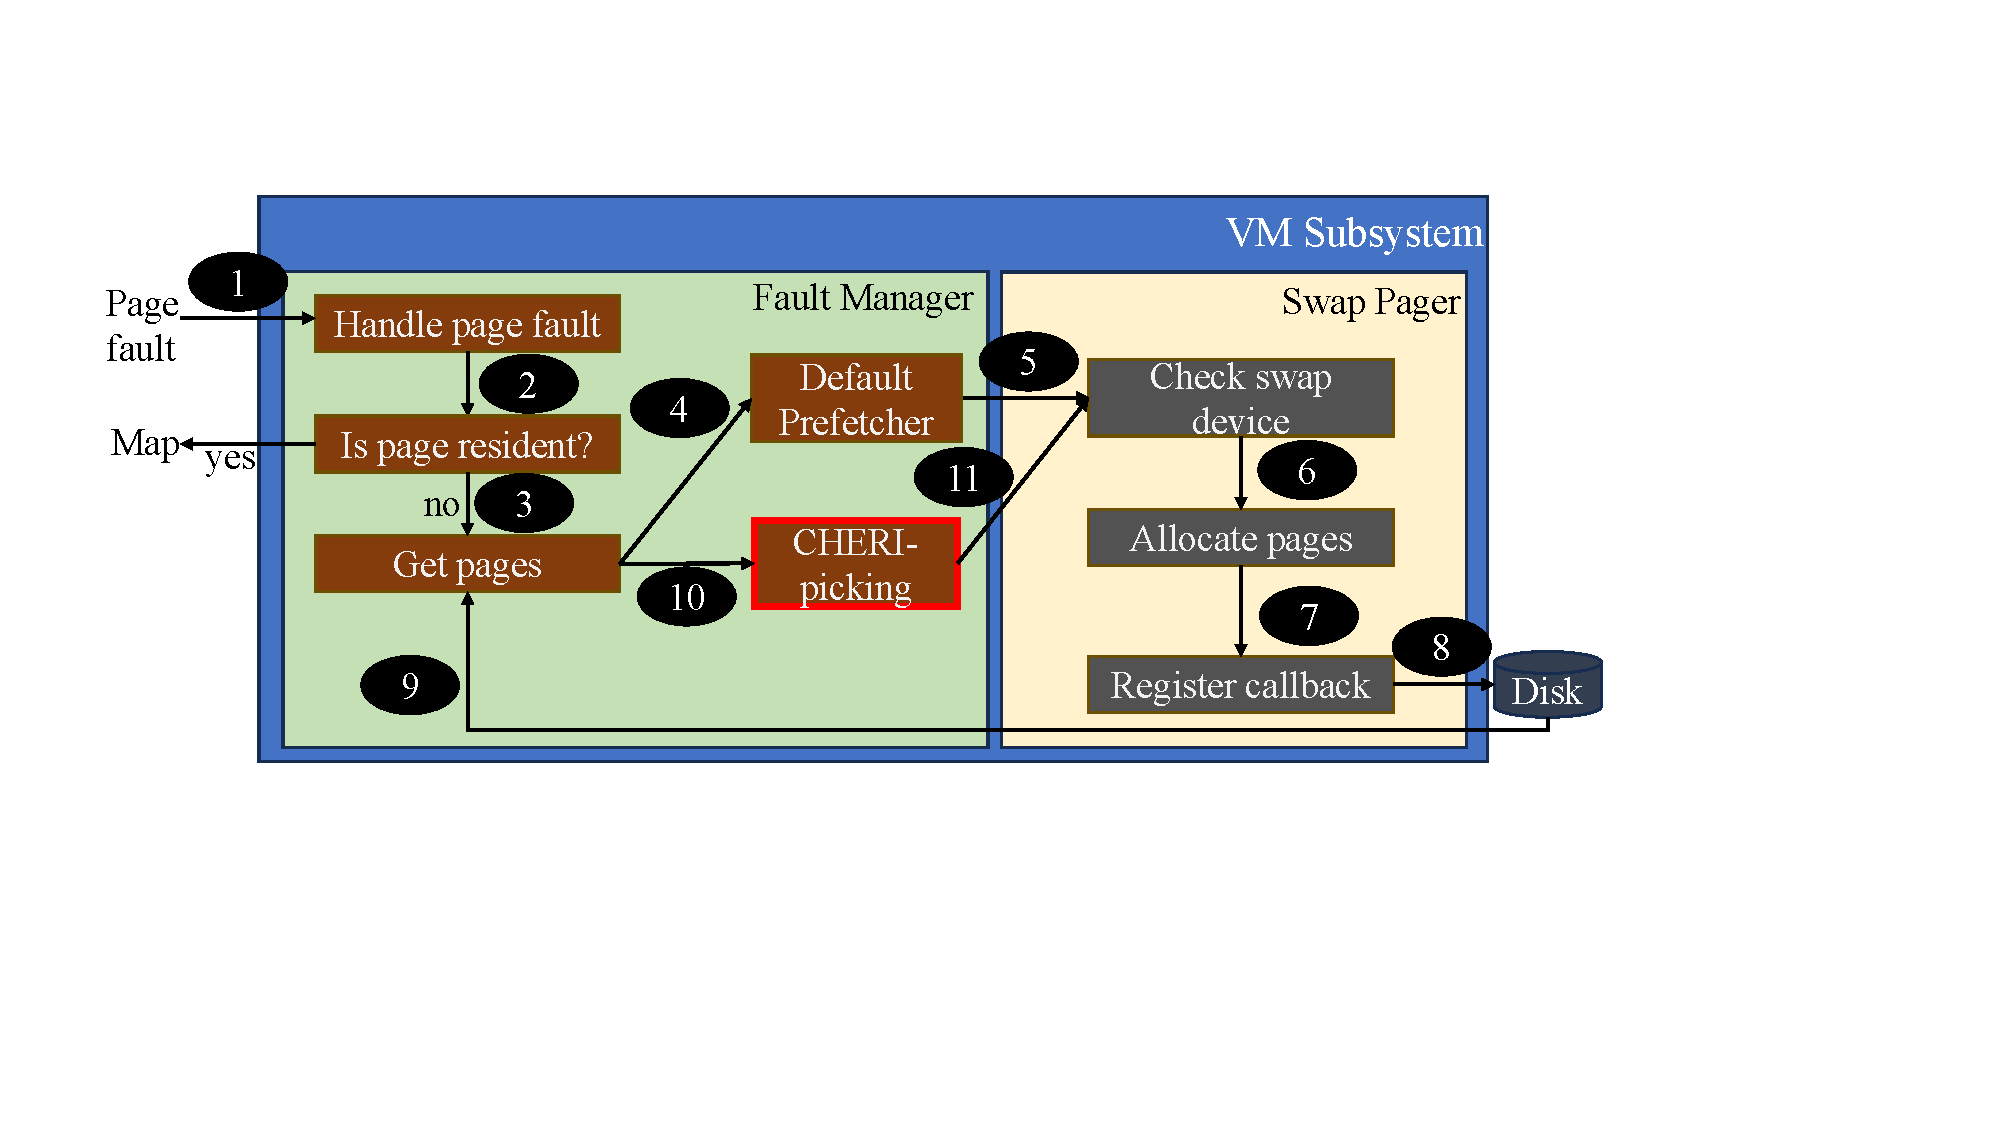
\includegraphics[width=\columnwidth]{images/CP_system_design_diagram.pdf}
\caption{CheriBSD swap workflow. 
CHERI-picking is invoked after the I/O request is completed.}
\label{fig:system_design}
\end{figure}

% Link the image 
% https://ubcca-my.sharepoint.com/:p:/g/personal/siagraw_student_ubc_ca/EWOPIZMY4VFIgUMZnJHmEu8B1EkDqDdvwLo2jrhZgjsXHQ?e=nWZW44
\autoref{fig:system_design} illustrates the high-level design of the CheriBSD swapping workflow; the numbers in this section refer to the figure. 
When a page fault occurs (\#1), the operating system checks if the page is already in memory (\#2). 
If it is, CheriBSD maps the page into the application's address space and resumes application execution; this is known as a \textbf{soft fault}.

If the page is not present in memory, the OS must retrieve the page from swap (in this case, the disk); this is called a \textbf{major fault}. The page fault dispatches a request to get pages (\#3). While getting the pages, the kernel executes the default prefetcher to detect sequential accesses (\#4). If the prefetcher detects a pattern, it checks if the requested page is present in the swap device (\#5). 
If the requested page is in swap, it prepares for prefetching by allocating physical frames~ (\#6).
It registers a callback for prefetched pages to put them into appropriate page queues when their I/O requests are completed (\#7).
Then it finally issues an I/O request for the faulting page and any pages to be prefetched (\#8). 
The swap manager returns after the faulting page is swapped in. 

%Previous works~\cite{canvas, dilos} invoke application-level pointer prefetchers during page faults, and CHERI-picking also adopts this as the initial design choice. This approach provides the OS with insight into application execution and a starting point for making prefetch decisions.


% After the faulting page is swapped in, the kernel invokes CHERI-picking. If, upon analyzing the page, the CHERI prefetcher discovers pointers to pages that are swapped out, it initiates their prefetching. Once the prefetcher completes these tasks, application execution resumes.

% I removed this stuff from the design because this seems to be related work.
 %CHERI-picking utilizes the contents of the faulted page to chase pointers, so we run it after the faulting page has been brought to memory. In the present design we do not  store pointer metadata of the swapped-out page separately from the page, so we must wait for the page to be swapped back in, so that we can find pointers
 %However, recent work~\cite{leap} has demonstrated that batching can have a negative impact in a disaggregated environment.
 %Application-level pointer prefetchers typically dispatch pointer requests to userspace when the kernel prefetcher either cannot make decisions or begins making faulty decisions.
 % In those works, specialized prefetchers were developed inside the application to use application knowledge to chase pointers through memory. 
 % The design of the CHERI-picking policy is similar to previous works~\cite{dilos, cache-analysis}.

\subsection{CHERI-picking policy} 
\label{sec:DI_CP_Policy}
% This needs a bit more work if we want to explain that we create a new capability in the kernel to look at the page.
CHERI-picking is highly configurable. We begin with an overview of when CHERI-picking is invoked, a description of the algorithm, and then discuss some key parameters available for tuning and future research. 
CHERI-picking does not change the CheriBSD page fault path at all.
Instead, after the callback for the faulting page occurs (\#9); CHERI-picking runs (\#10),
%it scans the page, checking the capability on each address in the faulting page \circled{10}
and according to configuration parameters, prefetches some pages (\#11)

%Recall from ~\autoref{sec:2} that CHERI’s pure cap compilation mode ensures that every pointer in an application is tagged by the hardware and treated as a capability. Thus, CHERI-picking works only on applications compiled in purecap mode.



\autoref{alg_1} describes the CHERI-picking algorithm. When the system swaps in a page, it obtains the kernel address for the physical page and iterates through its contents (lines 1-3). 
%The prefetcher starts at the beginning of the page and examines the entire page for pointers. 
For each address, CHERI-picking queries the hardware to retrieve the tag bit to determine if the address contains a pointer (line 4). 
Upon finding a pointer, it confirms that the page is not already present in memory or prefetched (line 6-7). 
It then verifies if the corresponding page is present in swap (line 8). 
If the page is present in swap it is added to an asynchronous prefetch queue (line 9), and the swap manager fetches these pages into main memory. We prefetch a fixed number of pages, a parameter called \textit{prefetch\_count} (line 3), which can be tuned. We could limit ourselves to prefetching a small number of pages, pages whose pointers reside in certain ranges on the page, or addresses that meet any desired or learned criteria. CHERI-picking could also run on soft faults. We leave this kind of policy exploration for future work (\autoref{sec:6}).

% OTHER POLICIES 
% Which direction to explore? Currently, we only explore down the page, but exploring before the currently faulted address might be beneficial for some applications
% Starting prefetching at the faulted addr rather than the top of the page is an obvious thing to explore 

\begin{algorithm}
\begin{algorithmic}[1]
\Require $faulting\_page$, $prefetch\_count$
\State $page\_addr \gets kernel\_addr(faulting\_page)$
%\State $page\_end \gets page\_addr + page\_size$
%\State $kernel\_capability \gets cheri\_setbounds(page\_addr, page\_size)$
\While{$page\_addr < page\_addr + page\_size$ AND \\
    \hspace{0.8cm} $ count < prefetch\_count \:$}
    \State $is\_ptr \gets cheri\_gettag(*page\_addr)$
    \If{$is\_ptr$} 
        %\State $page\_allocated \gets lookup\_vm\_map()$
        \If{$!page\_in\_ram()$ AND \\ 
            \hspace{1.45cm}$!page\_prefetched()$}
            \If{$page\_in\_swap()$}
                \State $get\_page\_async()$
                \State $count++$
            \EndIf
        \EndIf
    \EndIf
    \State $page\_addr~+= sizeof(CHERI\_Cap)$ \Comment{16 bytes}
\EndWhile
\end{algorithmic}
\caption{CHERI-picking algorithm}\label{alg:cheri}
\label{alg_1}
\end{algorithm}

\subsection{CHERI-picking design}
\label{sec:DI_CP_design}
We chose to implement CHERI-picking as a standalone function invoked by the callback to isolate our implementation during development and evaluation.
This has several consequences and suggests directions for future work.

Rather than implementing CHERI-picking in the swap callback function, one could merge CHERI-picking with the CheriBSD function 
\texttt{swp\_pager\_meta\_cheri\_get\_tags()} that restores a page's capabilities~\cite{cheri_get_tags}.
While we have not yet done that, this will likely reduce CHERI-picking's runtime overhead penalty, as discussed in
~\autoref{sec:overhead}.

Recall from ~\autoref{sec:2} that CHERI’s purecap compilation mode ensures that every pointer in an application is tagged by the hardware and treated as a capability. Thus, CHERI-picking works only on applications compiled in purecap mode.

As currently implemented, CHERI-picking always runs after the default prefetcher. 
On one hand, CHERI-picking detects, and prefetches accesses that the default prefetcher cannot. 
On the other hand, sometimes (as we’ll see in the microbenchmark results in ~\autoref{sec:5.1}), this can disrupt the performance of the default prefetcher.
Better communication between the default prefetcher and CHERI-picking should be able to remedy this.


\begin{comment}
% Why we run cheripicking at major fault?
% Why we run cheripicking after the page is swapped in?
% What does cheri-picking run for?
% % Why we run cheripicking at major fault?
CHERI-picking doesn't change the code path at all. Instead, it runs when the callback for the faulting page occurs; it scans the page, checking the capability on each address in the faulting page, and according to configuration parameters, prefetches a selection of them. We implemented CP as a standalone module invoked by the callback to isolate our implementation during development and evaluation. This has several consequences and suggests directions for future work. 

CHERI-picking makes prefetching decisions at major fault time. Prefetching at major fault time enables CHERI-picking to consider the context of application execution. We assume that spatial locality holds, indicating that pointers on the currently faulted page will likely be accessed soon. Further optimizations, such as prefetching at soft faults and performing pointer chasing in the kernel, are left as future work.

% Why we run cheripicking after the page is swapped in?
The default kernel prefetcher utilizes the memory access trace to make prefetching decisions. This trace is available prior to dispatching a request for the currently faulted page to disk, allowing for batching of sequential prefetching requests with the currently faulted page. In this situation, CHERI-picking distinguishes itself from the default prefetcher. In our current implementation, the request for the currently faulted page is sent to disk before CHERI-picking can execute the prefetcher. This is necessary as CHERI-picking needs to read the contents of the faulted page to find the pointers on the page. Currently, CHERI-picking always makes prefetching requests regardless of the default prefetchers decisions and requests pages that were potentially missed by the default prefetcher.

% What does cheri-picking run for?
CHERI-picking runs  for applications complied in \texttt{purecap} (see Section ~\ref{sec:2}) compilation mode, thus every pointer of an application is tagged by the hardware and treated as a capability. This allows CHERI-picking to run in an application-agnostic manner without the need for application hints.
\end{comment}








% TODO:
%Explian: cheri_gettag, page_in_ram, page_in_swap

\begin{comment}
\textbf{CheriBSD Policy Implementation:} 
To retrieve the tag from the metadata, $cheri\_gettag()$ utilizes a CHERI instruction. The prefetcher accesses CheriBSD's $vm\_map$, which contains a virtual address to $vm\_object$ mapping. Once the existence of the $vm\_object$ is confirmed, the prefetcher looks up the corresponding $pmap$, which maps $vm\_object$ to physical pages. The prefetcher sends prefetch requests to the swap pager, handling one page at a time. Although the prefetcher can batch multiple requests, our current focus is on increasing the VM cache hit rate. Optimizing disk accesses is left for future work.
\end{comment}